\documentclass[main.tex]{subfiles}

\begin{document}
This is the homework from problem set 1. This document was generated using
\LaTeX. If you have any questions feel free to contact me at nharvey@spsu.edu.

\begin{enumerate}

		%problem 2
		\setcounter{enumi}{1}
	\item
		\begin{enumerate}
				%2.a
			\item 
				\begin{align*}
					c(t) &= \Lapinv{R(s)G(s)}
					\\   &= 5\Lapinv{\frac{1}{s+5}\cdot\frac{1}{s}}
					\\   &= \boxed{u(t) - e^{-5t}}
				\end{align*}
				\begin{align*}
					T = \frac{1}{5}, T_r = \frac{2.2}{5}, T_s = \frac{4}{5}
				\end{align*}

				%2.b
			\item 
				\begin{align*}
					c(t) &= \Lapinv{R(s)G(s)}
					\\   &= \Lapinv{\frac{20}{s+20} \cdot \frac{1}{s}}
					\\   &= \boxed{u(t) - e^{-20t}}
				\end{align*}
				\begin{align*}
					T = \frac{1}{20}, T_r = \frac{2.2}{20}, T_s = \frac{1}{5}
				\end{align*}
		\end{enumerate}

		%problem 4
		\setcounter{enumi}{3}
	\item
		\begin{align*}
			5 - I(s)(R_1s+\frac{1}{Cs}) = 0
			\\\frac{I(s)}{5} = \frac{1}{R_1+\frac{1}{Cs}}
			\\\because \frac{I(s)}{V_c(s)} = \frac{1}{Cs}
			\\\therefore I(s) = V_c(s)Cs
			\\\therefore V_c(s) = \frac{5}{CR_1s+1}
			\\ \boxed{V_c(s) = \frac{\frac{10}{F}}{s+\frac{2}{F}}}
		\end{align*}
		\begin{align*}
			T = \frac{F}{2}, T_r = 1.1F, T_s = \frac{2}{F}
		\end{align*}

		% problem 8
		\setcounter{enumi}{7}
	\item
		\begin{enumerate}
				%8.a
			\item
				$C(s) = \frac{2}{s^2+2s}$, critically damed (this is a first order
				system), poles: $[-2]$, no zeros
				\\\begin{figure}[H]
					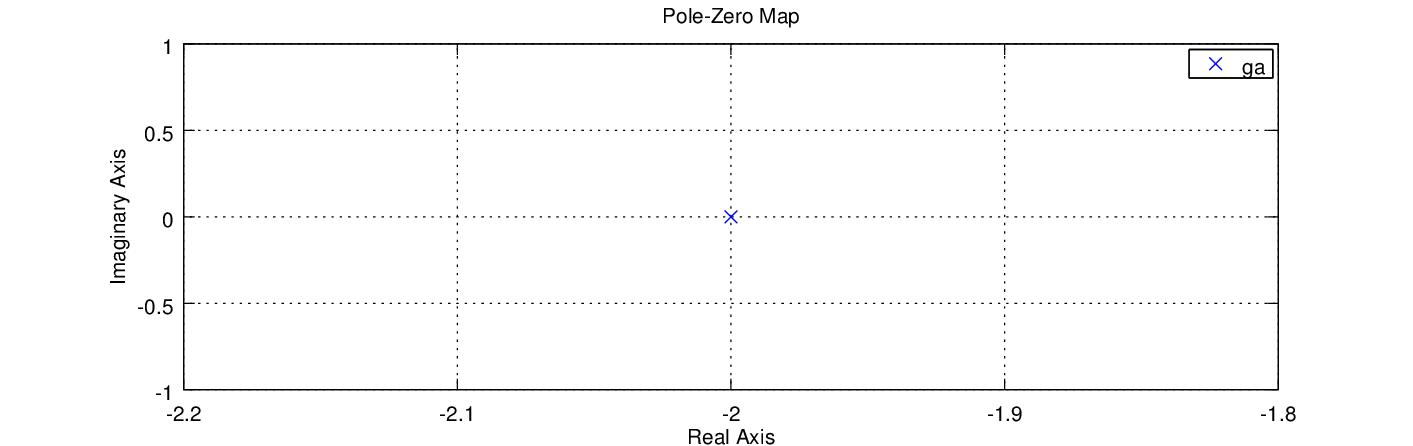
\includegraphics[width=\textwidth]{prob8a}
				\end{figure}

				%8.b
			\item
				$C(s) = \frac{20}{s(s^2+gs+144)}$, underdamped, poles: $-3 \pm 11.619j$,
				no zeros.
				\\\begin{figure}[H]
					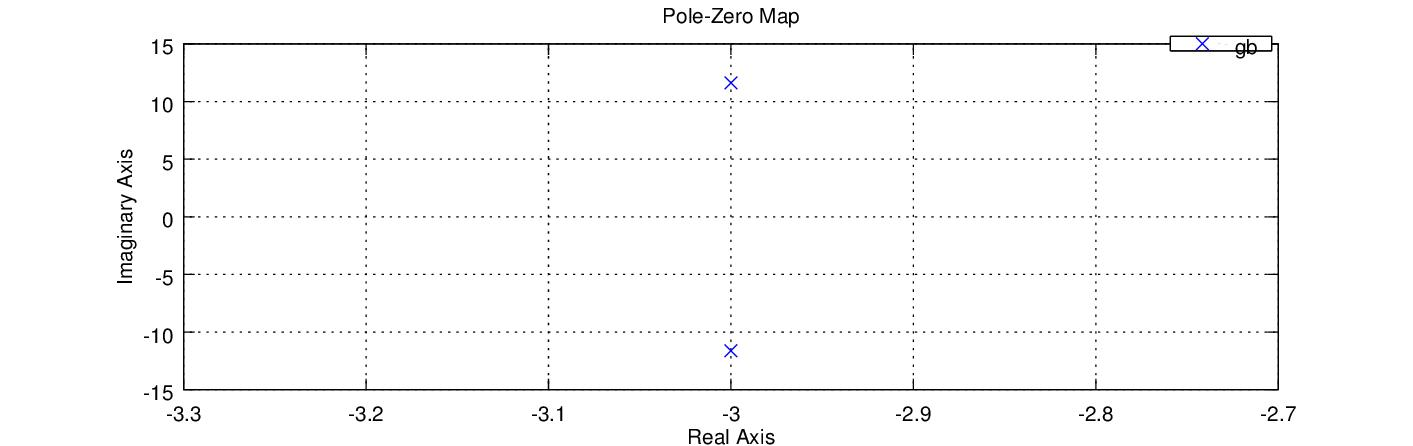
\includegraphics[width=\textwidth]{prob8b}
				\end{figure}

			\item
				$C(s) = \frac{(s+5)}{s(s+10)^2}$, critically damped, poles: $-10$,
				zeros: $-5$.
				\\\begin{figure}[H]
					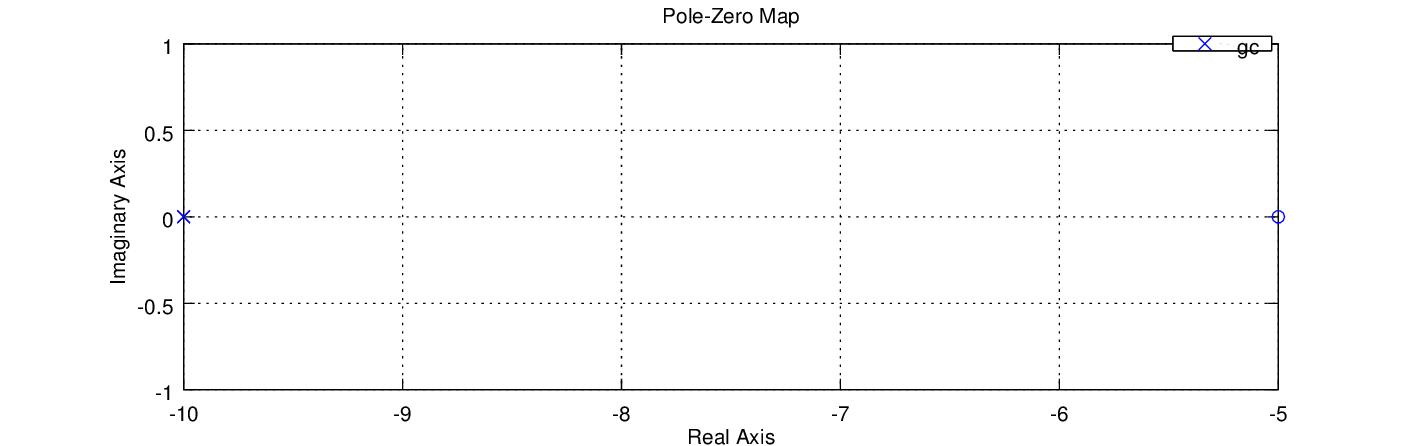
\includegraphics[width=\textwidth]{prob8c}
				\end{figure}
		\end{enumerate}

	%problem 17
	\setcounter{enumi}{16}
	\item
		\begin{enumerate}
			\item 
				\begin{align*}
					c(t) = u(t) - e^{-2t}
				\end{align*}
			\setcounter{enumii}{3}
			\item 
				$c(t) = a + be^{-3t}\cos{(11.619t+\phi)}$ (matlab required)
			\setcounter{enumii}{5}
			\item
				\begin{align*}
					c(t) &= \Lapinv{\frac{20}{s(s^2+gs+144)}}
					\\   &= \Lapinv{
						\begin{bmatrix}
							a=\frac{1}{20} & b=\frac{1}{2} & c=\frac{-1}{20}
						\end{bmatrix}
						\begin{bmatrix}
							s^-1 \\ (s+10)^{-2} \\ (s+10)^{-1}
						\end{bmatrix}
					}
					\\  &= a\Lapinv{\frac{1}{s}} 
					+ b\Lapinv{\frac{1}{(s+10)^2}} 
					+ c\Lapinv{\frac{1}{(s+10)}}
					\\  &= \boxed{\frac{1}{20} + \frac{1}{2}t\e^{-10t} + \frac{-1}{20}\e^{-10t}}
				\end{align*}
		\end{enumerate}

	%problem 18
	\item
		\begin{enumerate}
				\setcounter{enumii}{3}
				\item $\xi = 0.25 , \omega_n = 12$
				\setcounter{enumii}{5}
				\item $\xi = 1, \omega_n = 10$
		\end{enumerate}

	%problem 20
	\setcounter{enumi}{19}
	\item
		$\xi = 0.05, \omega_n = 0.2, T_r = 56.569, T_p = 2.2242, \%OS = 0.85447$

	%problem 30
	\setcounter{enumi}{29}
	\item
		Pole Cancelation can be assumed. $\omega_n = \sqrt(5), \xi = 0.224, 
		T_s = 7.986, T_r = 1.23, T_p = 1.4116$
\end{enumerate}

\end{document}
